\section{Literature}

\begin{frame}{FE$^2$ via Machine Learning}
  \begin{minipage}{0.5\textwidth}
  \only<1-2>
  {
    \centering
    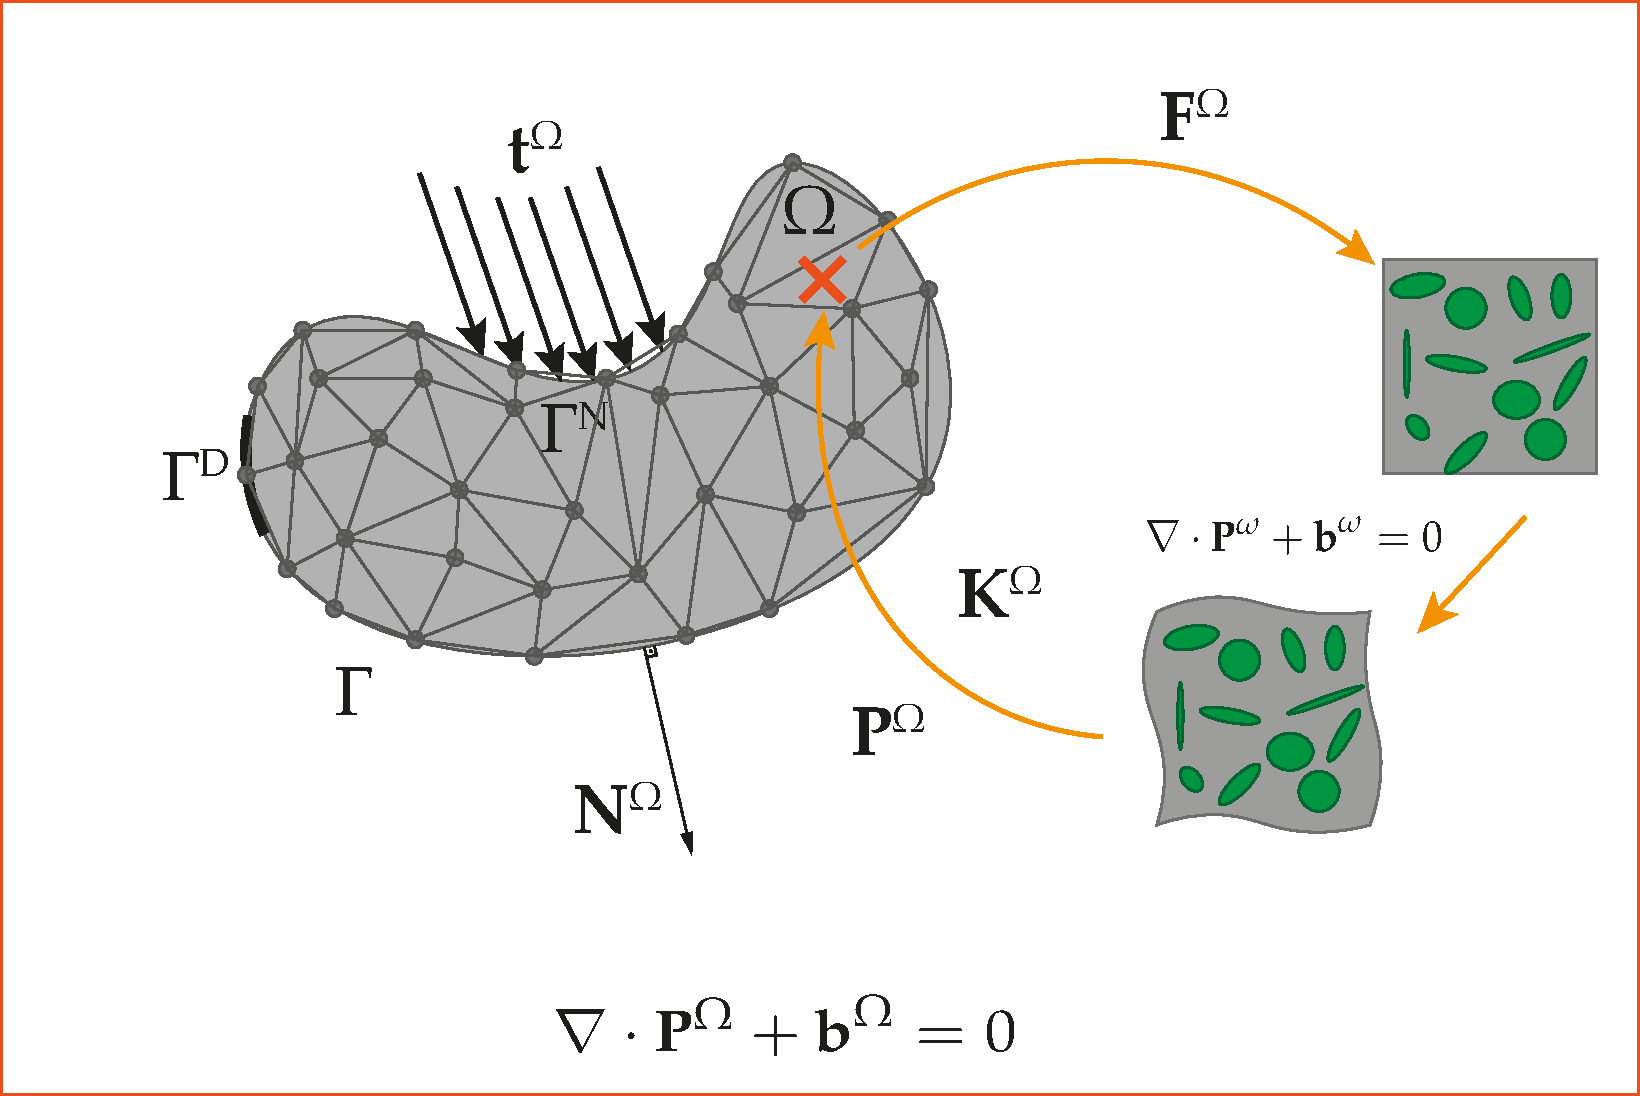
\includegraphics[width=0.9\textwidth]{Figures/intro/FE2-CONV}
  }
  \only<3>
  {
    \begin{block}{\color{White} Problems in Current State}
      \begin{itemize}
        \item Risky Extrapolation
        \item Data Scarcity
        \item Single Parameter Configuration
        \item General Applicability
      \end{itemize}
    \end{block}
  
  }
  \end{minipage}%
  \begin{minipage}{0.5\textwidth}
  \only<1-3>
  {
    \centering
    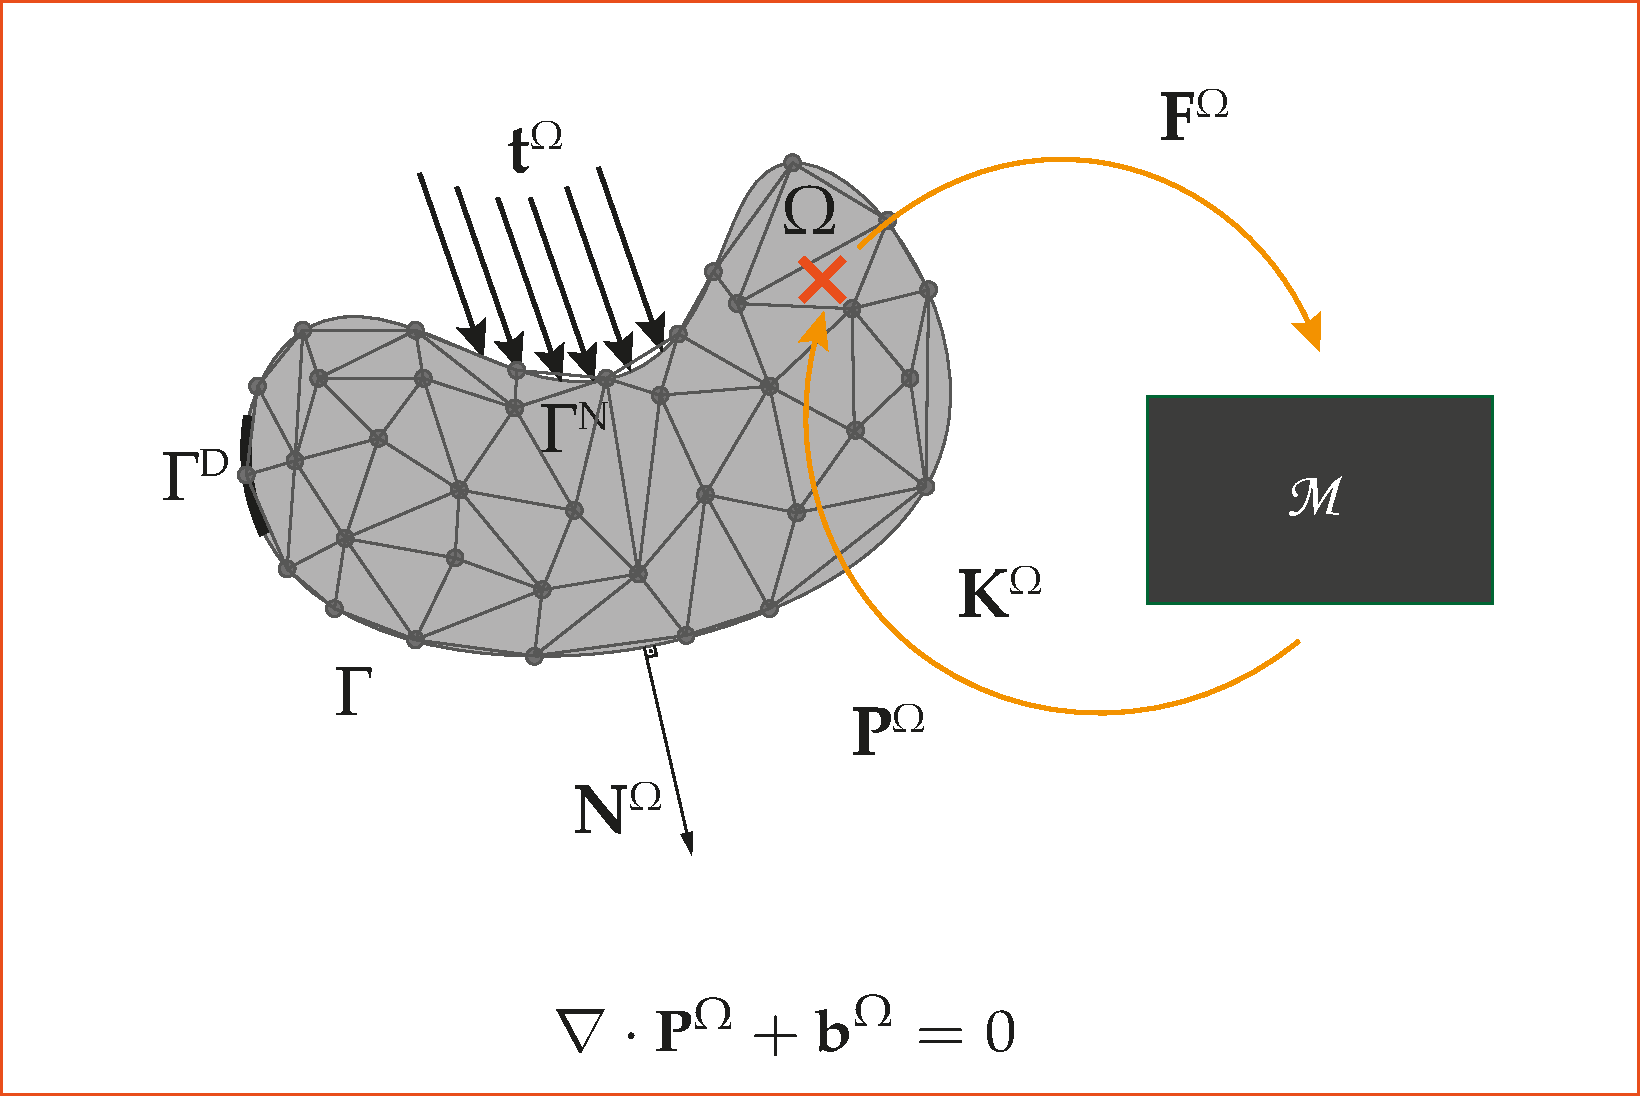
\includegraphics[width=0.9\textwidth]{Figures/literature/FE2-ML}
  }
  \end{minipage}
\only<2>
{
  \begin{itemize}
  \centering
    \item \color{Pink} Computationally a Material: $\mathbf{F} \to \mathbf{P}$
  \end{itemize}
}
\end{frame}

\begin{frame}{Hypothesis}
  \begin{itemize} 
    \item Most of the problems encountered can be tackled with more general approaches.
    \item The core problem is finding the mapping between a deformation measure and a force measure. ($\mathbf{P}=\mathcal{C}(\mathbf{F})$).
    \item Similarity between the problems can be exploited, without considering the different parameters that effect the model.
  \end{itemize}
\end{frame}






